\chapter{共形映射與開弦散射處方}

\lectureoverview{共形映射最初是二維靜電學中的一種實用對稱性。複可微性使這種對稱性變得可計算：柯西--黎曼方程蘊含拉普拉斯方程，而與方向無關的複導數會保持角度不變。有了這套工具，弦的世界面可以畫成條帶、半平面、圓柱或圓盤，物理內容都不因此改變。接著，開弦散射便可表示為圓盤上的高斯路徑積分，並在邊界插入動量，再對彼此不等價的插入位置積分。}

\section{二維世界中的靜電學}

我們先從字面意義上的二維靜電問題談起。電荷及其場線都局限在一個平面內；這些電荷並非只是運動恰好位於平面內的普通三維電荷。由高斯定律可得
\begin{equation}
  F(r)\propto \frac{1}{r},
  \qquad
  V(r)\propto \log r,
  \label{eq:l08-two-dimensional-coulomb}
\end{equation}
因為通量穿過一個圓，而圓周長隨\(r\)成正比地增加。

以標量位勢\(\phi\)表示電場。按照黑板上採用的符號慣例，
\begin{equation}
  \mathbf E=\nabla\phi,
  \qquad
  \nabla\cdot\mathbf E=\rho,
\end{equation}
因此
\begin{equation}
  \nabla^2\phi
  =\frac{\partial^2\phi}{\partial x^2}
  +\frac{\partial^2\phi}{\partial y^2}
  =\rho.
  \label{eq:l08-poisson}
\end{equation}
在無電荷區域，這便化為拉普拉斯方程：
\begin{equation}
  \nabla^2\phi=0.
  \label{eq:l08-laplace-phi}
\end{equation}
\editorialnote{許多電動力學教材採用定義
\(\mathbf E=-\nabla\Phi\)，因此吸收常數後，方程寫作
\(\nabla^2\Phi=-\rho\)。本講採用相反的位勢符號。無源方程及所有共形論證都不受影響。}

\begin{figure}[H]
  \centering
  \includegraphics[width=0.72\textwidth]{lecture_08_figure_01.png}
  \caption{靜電方程展開後成為二維泊松方程算子。}
  \lectureframe{00:03:48}
  \label{fig:l08-electrostatics-board}
\end{figure}

兩個空間導數之間的正號很重要：它使這個方程成為橢圓型方程，而非波動方程。共形變換會保持其無源形式，因此可以把某個區域上的解及其邊界條件映到形狀不同的區域。這種方法在弦理論之前，已廣泛用於靜電學、二維流體流動和製圖學。

\begin{classroomqa}
\audiencequestion{如果拉普拉斯算子為零，這是駐波方程嗎？\lecturetimestamp{00:05:35}}
\lecturerresponse{不是。兩個空間導數的符號相同，而且沒有時間導數。波動方程需要有時間依賴，且空間與時間項之間須具有洛侖茲度規的相對符號。靜電學之所以是靜態的，正是因為沒有任何東西在演化，波也不例外。}
\end{classroomqa}

\begin{classroomqa}
\audiencequestion{二維中有旋度嗎？
\lecturetimestamp{00:06:06}}
\lecturerresponse{有，但只有一個獨立分量。對於
\(\mathbf E=(E_x,E_y)\)，
\[
  \operatorname{curl}_{2d}\mathbf E
  =\partial_yE_x-\partial_xE_y.
\]
可以把它想成垂直於黑板的分量；不過，內在維度只有二維的世界並不需要外部的垂直方向。在更高維度中，相應的量自然是反對稱二形式。}
\end{classroomqa}

\section{沒有偏好方向的導數}

在原平面與像平面上引入複座標：
\begin{equation}
  z=x+iy,
  \qquad
  w=u+iv,
  \qquad
  w=w(z).
  \label{eq:l08-complex-coordinates}
\end{equation}
這裡的\(x,y,u,v\)都是實數。在局部，導數應為
\begin{equation}
  \frac{dw}{dz}
  =\lim_{\Delta z\to0}\frac{\Delta w}{\Delta z}.
  \label{eq:l08-complex-derivative}
\end{equation}
複平面不同於實數線，可以從無窮多個方向趨近某一點。即使映射連續且通常也很平滑，沿不同方向得到的比值仍未必相同。

比較兩種簡單的趨近方式。沿\(x\)方向，\(dy=0\)，因此
\begin{equation}
  \left.\frac{dw}{dz}\right|_x
  =\frac{\partial u}{\partial x}
  +i\frac{\partial v}{\partial x}.
\end{equation}
沿\(y\)方向，\(dx=0\)，且
\begin{equation}
  \left.\frac{dw}{dz}\right|_y
  =\frac{1}{i}\frac{\partial u}{\partial y}
  +\frac{\partial v}{\partial y}
  =\frac{\partial v}{\partial y}
  -i\frac{\partial u}{\partial y}.
\end{equation}
分別比較實部與虛部，得到
\begin{equation}
  \boxed{
  \frac{\partial u}{\partial x}
  =\frac{\partial v}{\partial y},
  \qquad
  \frac{\partial u}{\partial y}
  =-\frac{\partial v}{\partial x}}
  \label{eq:l08-cauchy-riemann}
\end{equation}
這就是柯西--黎曼方程。在通常的可微性假設下，這些方程也足以確保極限\eqref{eq:l08-complex-derivative}與趨近方向無關。在該點具有此性質的函數稱為解析函數，或全純函數。

\begin{figure}[H]
  \centering
  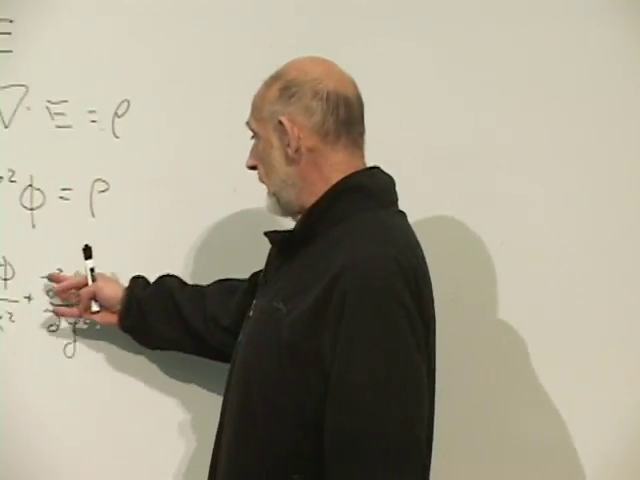
\includegraphics[width=0.70\textwidth]{lecture_08_figure_02.png}
  \caption{完整的柯西--黎曼方程組，包含相對的負號。}
  \lectureframe{00:19:48}
  \label{fig:l08-cr-board}
\end{figure}

本講也簡要區分幾個相關術語。在整個有限複平面上全純的函數稱為整函數；亞純函數則可以有孤立極點。因此，\(1/z\)在\(z=0\)之外解析，但不是整函數。

\section{調和共軛與共形幾何}

柯西--黎曼方程是耦合的一階方程，但它們也蘊含各自的二階方程。將\(\partial_xu=\partial_yv\)對\(x\)微分，將\(\partial_yu=-\partial_xv\)對\(y\)微分，再把兩式相加：
\begin{align}
  \partial_x^2u&=\partial_x\partial_yv,\\
  \partial_y^2u&=-\partial_y\partial_xv,\\
  \therefore\qquad
  \partial_x^2u+\partial_y^2u&=0.
  \label{eq:l08-harmonic-u}
\end{align}
交換\(u\)與\(v\)後重複同一論證，可得
\begin{equation}
  \partial_x^2v+\partial_y^2v=0.
  \label{eq:l08-harmonic-v}
\end{equation}
因此，解析函數的實部與虛部互為調和共軛。任意兩個調和函數不會自動組成解析函數；兩者仍須滿足\eqref{eq:l08-cauchy-riemann}所給的關係。

\begin{figure}[H]
  \centering
  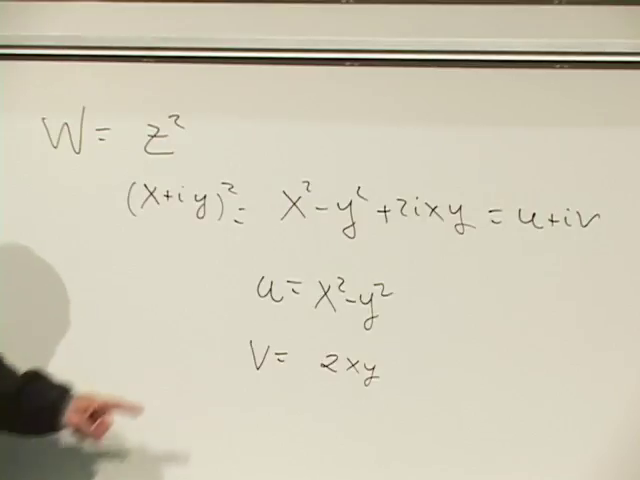
\includegraphics[width=0.68\textwidth]{lecture_08_figure_03.png}
  \caption{混合偏導數相消後，解析映射的一個分量便滿足拉普拉斯方程。}
  \lectureframe{00:23:09}
  \label{fig:l08-harmonic-board}
\end{figure}

還可以用向量來理解。若\(\mathbf F=(u,-v)\)，則兩個柯西--黎曼方程表示，在所採用的定向慣例下，\(\mathbf F\)的散度與二維旋度都為零。這就回到了靜電學。

\subsection{為何角度會保持不變}

將兩個微小的複位移寫成極式：
\begin{equation}
  \delta z=\rho e^{i\theta},
  \qquad
  \Delta z=\rho'e^{i\theta'}.
\end{equation}
兩者的比值相位為\(\theta-\theta'\)，恰好就是它們之間的夾角。在解析映射下，
\begin{equation}
  \frac{\delta w}{\delta z}
  =\frac{\Delta w}{\Delta z}
  =w'(z),
\end{equation}
因為導數與方向無關。重新整理可得
\begin{equation}
  \frac{\Delta z}{\delta z}
  =\frac{\Delta w}{\delta w}.
  \label{eq:l08-angle-ratio}
\end{equation}
等式兩側的相位相同，因此原來兩個線段的夾角，等於其映像之間的夾角。

\begin{figure}[H]
  \centering
  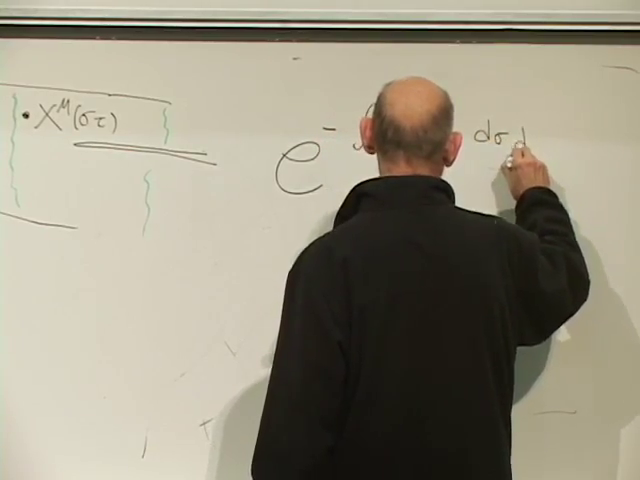
\includegraphics[width=0.70\textwidth]{lecture_08_figure_04.png}
  \medskip

  \begin{tikzpicture}[x=0.9cm,y=0.9cm,>=Latex]
    \begin{scope}
      \draw[->] (-0.2,0) -- (2.3,0);
      \draw[->] (0,-0.2) -- (0,2.1);
      \draw[very thick,blue!65!black,->] (0,0) -- (1.85,0.45)
        node[right] {\(\delta z\)};
      \draw[very thick,orange!75!black,->] (0,0) -- (0.72,1.65)
        node[above] {\(\Delta z\)};
      \draw (0.58,0.14) arc[start angle=14,end angle=66,radius=0.60];
      \node at (1.0,-0.55) {\(z\)-plane};
    \end{scope}
    \draw[->,thick] (3.0,0.9) -- (4.2,0.9)
      node[midway,above] {\(w(z)\)};
    \begin{scope}[xshift=5.0cm]
      \draw[->] (-0.2,0) -- (2.3,0);
      \draw[->] (0,-0.2) -- (0,2.1);
      \draw[very thick,blue!65!black,->] (0,0) -- (1.65,0.70)
        node[right] {\(\delta w\)};
      \draw[very thick,orange!75!black,->] (0,0) -- (0.48,1.62)
        node[above] {\(\Delta w\)};
      \draw (0.54,0.23) arc[start angle=23,end angle=74,radius=0.59];
      \node at (1.0,-0.55) {\(w\)-plane};
    \end{scope}
  \end{tikzpicture}
  \caption{黑板上的證明與清楚的局部重構。乘以\(w'(z)\)會讓每個無窮小方向都旋轉並縮放相同的量，因此相對角度保持不變。}
  \lectureframe{00:34:11}
  \label{fig:l08-angle-proof}
\end{figure}

這個局部論證假設\(w'(z)\neq0\)。在臨界點，映射可能不再是局部一對一，必須另行分析其幾何。離開這類點時，解析映射與保向的共形映射在局部上是同一類映射。

\section{幫助培養直覺的例子}

\subsection{平方映射與複共軛}

對於\(w=z^2\)，
\begin{equation}
  (x+iy)^2=x^2-y^2+2ixy=u+iv,
\end{equation}
因此
\begin{equation}
  u=x^2-y^2,
  \qquad
  v=2xy.
  \label{eq:l08-z-squared-components}
\end{equation}
\(u\)的二階導數為\(2\)與\(-2\)；\(v\)的二階導數則各自為零。兩者都是調和函數，直接微分也可驗證柯西--黎曼方程。

\begin{figure}[H]
  \centering
  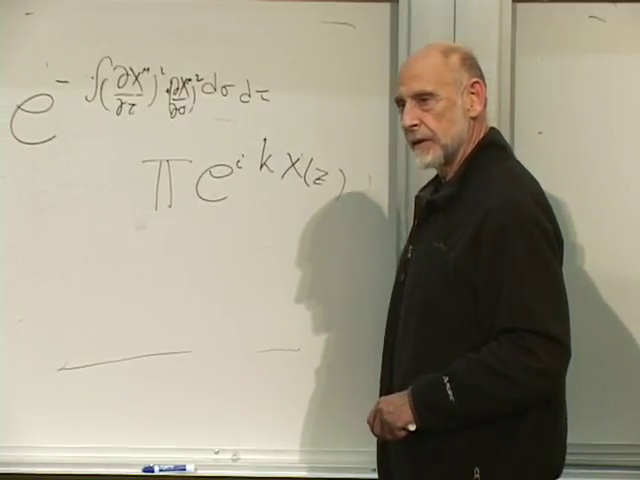
\includegraphics[width=0.72\textwidth]{lecture_08_figure_05.png}
  \caption{平方映射分解成實部與虛部兩個調和分量。}
  \lectureframe{00:36:45}
  \label{fig:l08-z-square-board}
\end{figure}

\begin{classroomqa}
\audiencequestion{\(1/z\)是非解析函數的例子嗎？
\lecturetimestamp{00:37:49}}
\lecturerresponse{只在一個點有問題。它在\(z\neq0\)處解析，而在原點有極點。若要看一個處處不滿足柯西--黎曼檢驗的映射，複共軛是更好的例子。}
\end{classroomqa}

相較之下，
\begin{equation}
  w=\bar z=x-iy
  \qquad\Longrightarrow\qquad
  u=x,\quad v=-y
\end{equation}
會反轉定向。它的導數因符號相反而不滿足第一個柯西--黎曼方程，因此它不是以\(z\)為自變數的解析函數。

\begin{figure}[H]
  \centering
  \includegraphics[width=0.62\textwidth]{lecture_08_figure_06.png}
  \caption{複共軛是刻意選用的非解析反例。}
  \lectureframe{00:38:38}
  \label{fig:l08-conjugate-board}
\end{figure}

\subsection{指數函數及其反函數}

\begin{classroomqa}
\audiencequestion{若\(e^z\)是解析函數，為何它的反函數\(\log z\)也應該是解析函數？\lecturetimestamp{00:40:38}}
\lecturerresponse{在反函數存在且\(w'(z)\neq0\)的地方，它的導數為\(1/w'(z)\)。因此，導數仍與方向無關。對數函數在整體上是多值的，所以必須選定一個分支，並排除其分支點與分支切線。在選定的區域內，局部共形的敘述仍然成立。}
\end{classroomqa}

尤拉公式給出
\begin{equation}
  w=e^z=e^{x+iy}
  =e^x(\cos y+i\sin y),
\end{equation}
因此
\begin{equation}
  u=e^x\cos y,
  \qquad
  v=e^x\sin y.
  \label{eq:l08-exponential-components}
\end{equation}
例如，\(\partial_xu=e^x\cos y=\partial_yv\)，第二個柯西--黎曼方程也可同樣直接得到。

\begin{figure}[H]
  \centering
  \includegraphics[width=0.68\textwidth]{lecture_08_figure_07.png}
  \caption{指數映射的實部與虛部。}
  \lectureframe{00:42:23}
  \label{fig:l08-exponential-board}
\end{figure}

\section{半平面、帶狀區域、圓柱與圓盤}

\subsection{對數將半徑轉為時間}

取右半平面，其中\(-\pi/2<\theta<\pi/2\)，並令
\begin{equation}
  z=re^{i\theta},
  \qquad
  w=\log z=\log r+i\theta.
  \label{eq:l08-log-map}
\end{equation}
右半平面便映到無限延伸的帶狀區域
\begin{equation}
  -\frac{\pi}{2}<\operatorname{Im}w<\frac{\pi}{2}.
\end{equation}
固定\(\theta\)的射線會變成水平線，固定\(r\)的半圓則會變成垂直線。原點映到\(\operatorname{Re}w=-\infty\)，而\(r=\infty\)映到\(\operatorname{Re}w=+\infty\)。

\begin{figure}[H]
  \centering
  \includegraphics[width=0.75\textwidth]{lecture_08_figure_08.png}
  \caption{對數將右半平面映入無限延伸的帶狀區域：極射線與半圓變成互相垂直的矩形網格。}
  \lectureframe{00:47:48}
  \label{fig:l08-log-strip-board}
\end{figure}

帶狀區域是開弦的標準世界面。有限範圍的座標是沿著弦的參數，而沿無限延伸方向的平移則代表世界面時間。透過反指數映射，時間平移會變成縮放\(z\mapsto e^a z\)。因此，同一個對稱性在帶狀區域中表現為平移，在半平面中則表現為均勻膨脹。

\begin{classroomqa}
\audiencequestion{像\(r=1\)這樣的特定值會映到哪裡？帶狀區域上的座標仍然是極座標嗎？\lecturetimestamp{00:50:58}}
\lecturerresponse{固定半徑的圓會變成\(\operatorname{Re}w=\log r\)處的垂直線；尤其是，\(r=1\)會映到中心線\(\operatorname{Re}w=0\)。極座標描述的是\(z\)平面；\(w\)平面則使用一般的直角座標\((\log r,\theta)\)。}
\end{classroomqa}

若以\(\log z\)映射整個穿孔平面，角座標的週期為\(2\pi\)。因此，所得帶狀區域的上、下邊緣會相互識別，形成無限長圓柱。帶有邊界的半平面描述開弦世界面；沒有邊界且角度具有週期性的整個平面，則描述閉弦圓柱。

\begin{figure}[H]
  \centering
  \includegraphics[width=0.75\textwidth]{lecture_08_figure_09.png}
  \caption{半平面與帶狀區域的圖像，以及將整個穿孔平面變成閉弦圓柱的週期性識別。}
  \lectureframe{00:54:23}
  \label{fig:l08-open-closed-board}
\end{figure}

\subsection{映至單位圓盤的凱萊映射}

線性分式映射，又稱莫比烏斯映射，可將右半平面映至單位圓盤：
\begin{equation}
  w=\frac{z-1}{z+1}.
  \label{eq:l08-cayley}
\end{equation}
它將\(z=0\)映至\(-1\)，將\(z=\infty\)映至\(+1\)，並將虛軸映至\(|w|=1\)。若\(z=ir\)，則
\begin{equation}
  \left|\frac{ir-1}{ir+1}\right|=1.
\end{equation}
滿足\(\operatorname{Re}z>0\)的點會映到圓內；左半平面則映到圓外。
\editorialnote{在現場推導中，描述圓盤內部映像時寫下了倒數\((z+1)/(z-1)\)。這個倒數有相同的單位圓邊界，但會將右半平面映到圓外。方程\eqref{eq:l08-cayley}採用的是與所述幾何相符的圓盤內部慣例。}

\begin{figure}[H]
  \centering
  \includegraphics[width=0.72\textwidth]{lecture_08_figure_10.png}
  \caption{構造單位圓邊界的線性分式映射。黑板上出現的倒數形式會交換圓內與圓外。}
  \lectureframe{00:58:38}
  \label{fig:l08-cayley-board}
\end{figure}

莫比烏斯映射會將廣義圓（包括直線）映成廣義圓。因此，半平面上的徑向線與圓弧網格，在圓盤上會變成兩族互相垂直的弧。直徑只是圓心趨於無窮遠時的圓弧極限。

\begin{classroomqa}
\audiencequestion{圓盤內畫出的弧真的都是圓嗎？
\lecturetimestamp{01:00:55}}
\lecturerresponse{是的。它們的圓心各不相同，而且常在可見圓盤之外。直徑就是同一族圓的半徑趨於無窮大時的極限。}
\end{classroomqa}

\begin{classroomqa}
\audiencequestion{圖中的圓盤代表球面嗎？另一個半平面映到哪裡？\lecturetimestamp{01:01:21}}
\lecturerresponse{這裡畫的是平面圓盤，不是球面。右半平面映到圓的內部，左半平面則映到圓外。若將無窮遠點加入整個複平面，擴充後的平面可透過球極投影表示為球面；那是另一個整體性的敘述。}
\end{classroomqa}

\begin{classroomqa}
\audiencequestion{圓盤中的哪些曲線對應於原本的徑向線與等半徑半圓？\lecturetimestamp{01:02:59}}
\lecturerresponse{正實軸會變成連接\(-1\)與\(+1\)的直徑。其他射線會變成連接這兩個邊界點的圓弧。等半徑半圓則變成另一族互相垂直、兩端落在單位圓上的曲線。}
\end{classroomqa}

\begin{figure}[H]
  \centering
  \includegraphics[width=0.72\textwidth]{lecture_08_figure_11.png}
  \caption{半平面中的直線與半圓，在圓盤中變成互相垂直的圓弧與直線族。}
  \lectureframe{01:03:48}
  \label{fig:l08-circle-grid-board}
\end{figure}

\section{四弦世界面}

現在回到散射。兩條開弦入射，合併成一條弦，傳播一段任意長的時間，再分裂成兩條出射弦。在帶狀座標中，世界面看起來像一條長帶子，兩端各開有一道縫---這就是「運動繃帶」的圖像。中間態的存續時間並非預先選定，而是振幅積分所涵蓋的各種歷程之一。

令\((\sigma,\tau)\)為世界面上的座標，並令
\begin{equation}
  X^\mu=X^\mu(\sigma,\tau)
  \label{eq:l08-embedding}
\end{equation}
表示世界面在時空中的位置。標記\(\sigma,\tau\)位於二維參數曲面上；指標\(\mu\)則標示時空座標。在玻色弦理論中，\(\mu=0,\ldots,25\)；超弦理論則有十個時空座標。

經過 Wick 轉動後，自由嵌入場的歐幾里得作用量為
\begin{equation}
  S_E[X]
  =\frac{1}{4\pi\alpha'}\int_\Sigma d\sigma\,d\tau\,
  \left[
    \partial_\tau X^\mu\partial_\tau X_\mu
    +\partial_\sigma X^\mu\partial_\sigma X_\mu
  \right].
  \label{eq:l08-euclidean-action}
\end{equation}
相應的路徑積分會對所選世界面嵌入時空的所有方式求和：
\begin{equation}
  \int\mathcal D X\,e^{-S_E[X]}.
  \label{eq:l08-bare-worldsheet-integral}
\end{equation}

\begin{figure}[H]
  \centering
  \includegraphics[width=0.74\textwidth]{lecture_08_figure_12.png}
  \caption{完整且為正的歐幾里得世界面權重。兩個導數項都對所有時空分量求和。}
  \lectureframe{01:11:34}
  \label{fig:l08-action-board}
\end{figure}

帶縫的條帶只有一個連通邊界。因此，利用共形自由度，可以將它表示為圓盤。條帶的四個遠端會變成邊界上的四個標記點。移動這些標記點會改變條帶座標中合併與分裂看起來相隔多遠，但不會改變底層曲面或物理內容。

\begin{figure}[H]
  \centering
  \includegraphics[width=0.76\textwidth]{lecture_08_figure_13.png}
  \caption{帶縫條帶世界面及其圓盤表示，外部弦對應到圓盤邊界上的點。}
  \lectureframe{01:15:18}
  \label{fig:l08-bandage-disc-board}
\end{figure}

用來描繪此共形映射的細部網格線沒有物理意義。重要的是拓撲、邊界和代表外部態的標記點。同一個世界面可以拉伸成不同的通道圖像，而無須引入新的交互作用。

\section{外部態作為邊界插入}

裸積分\eqref{eq:l08-bare-worldsheet-integral}尚未說明哪些動量入射、哪些動量出射。對動量為\(k_i^\mu\)的純量開弦態，在邊界上插入頂點算符
\begin{equation}
  V_i(z_i)=e^{\,i k_i\cdot X(z_i)},
  \qquad
  k_i\cdot X=k_{i\mu}X^\mu.
  \label{eq:l08-vertex}
\end{equation}
點\(z_i\)是世界面邊界上的位置；它不是時空座標，也不代表動量方向。

\begin{figure}[H]
  \centering
  \includegraphics[width=0.72\textwidth]{lecture_08_figure_14.png}
  \caption{體內的歐幾里得權重與邊界動量插入的乘積分別列為不同因子。}
  \lectureframe{01:18:58}
  \label{fig:l08-vertex-board}
\end{figure}

對\(n\)條外部開弦，示意性的散射處方為
\begin{equation}
  \begin{aligned}
    \mathcal A_n(k_1,\ldots,k_n)
    &=\int_{\mathcal M_{0,n}^{\partial}}\!d\mu(z_i)
      \int\mathcal D X\\
    &\quad\times e^{-S_E[X]}
      \prod_{i=1}^{n}e^{\,i k_i\cdot X(z_i)}.
  \end{aligned}
  \label{eq:l08-open-string-prescription}
\end{equation}
泛函積分是對嵌入場\(X^\mu\)進行；有限維積分則是對彼此不等價的邊界插入位置進行。此處省略了極化因子與規範固定測度，講課時也同樣省略。
\editorialnote{完整的規範固定弦振幅還包含相應的鬼場貢獻、依態而定的頂點因子、耦合常數及歸一化。方程\eqref{eq:l08-open-string-prescription}記錄的是本講所推導的嵌入場與位置依賴性。}

\begin{classroomqa}
\audiencequestion{既然外部動量固定，為什麼還要對它們積分？\lecturetimestamp{01:20:42}}
\lecturerresponse{外部動量並沒有被積分。\(k_i\)是散射振幅中的固定標記。被積分的是嵌入場，以及插入這些固定動量的世界面位置\(z_i\)。後者的積分取代了條帶圖像中對中間態存續時間的積分。}
\end{classroomqa}

\begin{classroomqa}
\audiencequestion{頂點因子的乘積放在路徑積分內；它是作用量的一部分嗎？\lecturetimestamp{01:21:39}}
\lecturerresponse{這些因子乘在泛函積分中的\(e^{-S_E}\)上。也可以把因子等價地併入指數，視為加入作用量的局域源項；不過在概念上，它們是頂點算符，而非自由的體作用量的一部分。}
\end{classroomqa}

\begin{figure}[H]
  \centering
  \includegraphics[width=0.76\textwidth]{lecture_08_figure_15.png}
  \caption{以彼此分開的因子\(e^{ik_i\cdot X(z_i)}\)表示每個外部粒子的路徑積分。}
  \lectureframe{01:23:23}
  \label{fig:l08-full-prescription-board}
\end{figure}

\begin{classroomqa}
\audiencequestion{世界面 Wick 轉動後，\(e^{ik\cdot X}\)為什麼仍含有\(i\)？\lecturetimestamp{01:23:42}}
\lecturerresponse{轉動改變的是世界面時間，並將體內權重從\(e^{iS}\)轉為\(e^{-S_E}\)。動量本徵函數中的\(i\)則是標記時空動量的傅立葉相位，作用不同，因此仍然保留。}
\end{classroomqa}

\begin{classroomqa}
\audiencequestion{位置\(z_i\)會決定動量向量的方向嗎？\lecturetimestamp{01:24:19}}
\lecturerresponse{不會。方向由時空分量\(k_i^\mu\)表示。插入點\(z_i\)說明該動量在世界面描述中的插入位置；\(X^\mu(z_i)\)則是由\(\mathcal D X\)所求和的場值之一。}
\end{classroomqa}

\begin{classroomqa}
\audiencequestion{圖中繃帶兩端的傾斜角度，代表物理動量的方向嗎？\lecturetimestamp{01:25:07}}
\lecturerresponse{不代表。繃帶描繪的是參數空間，不是弦在物理時空中的形狀。兩端可以畫成水平、傾斜，或經共形變換而彎曲。物理方向由分量\(k^\mu\)表示，而\(X^\mu(\sigma,\tau)\)則是積分變數。}
\end{classroomqa}

\section{高斯積分與靜電學}

作用量\eqref{eq:l08-euclidean-action}對每個\(X^\mu\)分量都是二次的；將插入算符的指數因子與作用量合併後，插入便形成線性源。因此，泛函積分是高斯積分。在鞍點處，每個時空分量都滿足泊松方程，其示意形式為
\begin{equation}
  \nabla^2 X^\mu(z)
  \propto
  i\alpha'\sum_i k_i^\mu\,\delta(z-z_i),
  \label{eq:l08-electrostatic-source}
\end{equation}
並在圓盤邊界上滿足開弦的邊界條件。每個\(X^\mu\)都像是各自獨立的靜電位勢，而每個動量分量\(k_i^\mu\)則像是置於\(z_i\)的相應電荷。

\begin{figure}[H]
  \centering
  \includegraphics[width=0.76\textwidth]{lecture_08_figure_16.png}
  \caption{帶有邊界源的圓盤，可解讀為每個時空分量各自對應一個獨立的二維靜電問題。}
  \lectureframe{01:28:58}
  \label{fig:l08-electrostatic-disc-board}
\end{figure}

先解出靜電問題並計算其能量，再取負能量的指數，最後對彼此不等價的電荷位置積分。在標準開弦歸一化下，嵌入場的關聯函數給出 Koba--Nielsen 因子
\begin{equation}
  \left\langle\prod_i e^{\,ik_i\cdot X(z_i)}\right\rangle
  \propto
  (2\pi)^D\delta^{(D)}\!\left(\sum_i k_i\right)
  \prod_{i<j}|z_i-z_j|^{2\alpha' k_i\cdot k_j}.
  \label{eq:l08-koba-nielsen}
\end{equation}
狄拉克 delta 函數表示動量守恆。乘積中的各項包含成對的靜電能。對於此處使用的四個純量邊界插入，固定三個位置後，剩下的積分便化為前幾講介紹過的尤拉 beta 積分。

\begin{classroomqa}
\audiencequestion{靜電能是有二十六個，還是只有一個？
\lecturetimestamp{01:30:53}}
\lecturerresponse{每個時空分量都對應一個獨立的位勢與電場。在正交歸一的靶空間基底中，各分量的二次能量沒有交叉項；取指數之前，所有貢獻會先加總成一個總作用量。}
\end{classroomqa}

\begin{classroomqa}
\audiencequestion{圓盤上的角座標就是物理散射角嗎？\lecturetimestamp{01:32:10}}
\lecturerresponse{不是。它是世界面上的位置參數。其不等價組合與中間傳播時間有關，並且需要積分。物理散射角則由固定動量所構成的洛侖茲不變量來表示。}
\end{classroomqa}

\begin{classroomqa}
\audiencequestion{為什麼這個構造在臨界維度以外會失效？
\lecturetimestamp{01:32:35}}
\lecturerresponse{形式上的高斯積分並不足以確保理論一致。規範固定會引入共形反常；只有在臨界維度，物質場與鬼場的貢獻才會相消：玻色弦為\(D=26\)，超弦為\(D=10\)。若未能相消，量子世界面所假設的共形對稱性便會消失。}
\end{classroomqa}

\begin{classroomqa}
\audiencequestion{我們是否已經假設有三個宏觀空間維度，以及緊緻化的額外維度？\lecturetimestamp{01:33:38}}
\lecturerresponse{沒有，這個構造尚未涉及緊緻化。在此階段，玻色弦的座標仍涵蓋靶空間的全部二十六個方向；超弦則涵蓋十個方向。如何讓其中一部分維度在宏觀尺度上保持廣延，會在接下來的討論中說明。}
\end{classroomqa}

\begin{classroomqa}
\audiencequestion{這裡與靜電學的關聯，是否只在於座標滿足拉普拉斯方程？\lecturetimestamp{01:33:57}}
\lecturerresponse{正是如此。在插入點以外，每個\(X^\mu\)都是調和的；頂點算符則提供 delta 函數源。無論是否使用靜電學的說法，這在數學上都與帶有點電荷的靜態二維位勢邊值問題相同。}
\end{classroomqa}

\subsection{共形冗餘與模數的數目}

圓盤的共形自同構群有三個實參數，為\(\mathrm{PSL}(2,\mathbb R)\)。因此，可以將三個有序的邊界點固定在方便的位置。對於四條外部弦，只剩第四個位置需要積分；對於\(n\)個有序邊界插入，樹圖階的實位置積分有
\begin{equation}
  n-3
  \label{eq:l08-n-minus-three}
\end{equation}
個。

\begin{classroomqa}
\audiencequestion{圓盤周圍有四個彼此獨立的角位置嗎？\lecturetimestamp{01:34:37}}
\lecturerresponse{物理上並非如此。起初雖然寫下四個位置，但圓盤的共形對稱性可以把任意三個位置選在方便之處。對於兩條入射、兩條出射的振幅，只剩第四個位置相對於其他位置的關係需要考慮。}
\end{classroomqa}

\begin{figure}[H]
  \centering
  \includegraphics[width=0.72\textwidth]{lecture_08_figure_17.png}
  \caption{圓盤上的四個邊界插入。共形自由度可固定任意三個位置，留下四點的一個模數。}
  \lectureframe{01:35:18}
  \label{fig:l08-fix-three-board}
\end{figure}

\begin{classroomqa}
\audiencequestion{如果條帶圖中的兩個分裂點不在同一高度，會怎樣？\lecturetimestamp{01:35:24}}
\lecturerresponse{共形映射可以消除這種表面上的高度差異。不同圖像只是同一模數的不同座標表示。真正不變的積分是對剩餘邊界位置積分，也等價於對傳播時間積分。}
\end{classroomqa}

\begin{classroomqa}
\audiencequestion{外部粒子更多時，還剩下多少個位置參數？\lecturetimestamp{01:36:00}}
\lecturerresponse{利用共形對稱性固定三個插入點，再對其餘\(n-3\)個位置積分。這就是有序樹圖階開弦振幅的邊界模數計數。}
\end{classroomqa}

\begin{classroomqa}
\audiencequestion{這和 M 理論有什麼關係？
\lecturetimestamp{01:36:37}}
\lecturerresponse{目前還沒有。這裡討論的是世界面上的微擾開弦散射。它與 M 理論的關係需要借助後續的對偶性與非微擾觀念，因此這個問題留待之後討論。}
\end{classroomqa}

\begin{classroomqa}
\audiencequestion{不同的垂直或交叉條帶圖示，代表不同的計算嗎？\lecturetimestamp{01:36:49}}
\lecturerresponse{不是。可以固定一個方便的點，讓其餘模數在完整的區間內變化。條帶圖示與圓盤上的邊界點積分，是同一積分的不同切片方式；因此，所有外部弦都能以對稱的方式處理。}
\end{classroomqa}

\section{此處方尚未解決的問題}

圓盤公式可直接推廣至更多外部弦：加入更多頂點算符，並對其 \(n-3\) 個互不等價的邊界位置積分。這是針對自洽弦模型的精確樹級處方，但還不是描述已觀測粒子物理的現實模型。簡單的玻色弦理論有錯誤的時空維度，並存在其他物理缺陷。超弦改善了粒子譜，並將臨界維度降至十維，但仍須將六個空間維度緊緻化。

\begin{classroomqa}
\audiencequestion{這個簡單模型已經符合粒子碰撞實驗嗎？\lecturetimestamp{01:39:06}}
\lecturerresponse{還沒有。它的共振結構在歷史上與強子散射相似，但二十六維玻色弦模型無法直接描述已觀測到的粒子。這套形式架構為該模型定義了散射振幅；若要符合自然界，還需要現實的粒子譜、緊緻化、交互作用以及真空選擇。}
\end{classroomqa}

\begin{classroomqa}
\audiencequestion{緊緻化能縮減額外維度，並產生符合現實的粒子資料嗎？\lecturetimestamp{01:41:10}}
\lecturerresponse{緊緻化可以降低有效的宏觀維度，並產生粒子譜與規範群。許多數學上的真正困難也由此而來。已有許多自洽的緊緻化方案，但如何選出唯一能描述已觀測基本粒子的模型，仍未有定論。}
\end{classroomqa}

本講強調這項區別，而非宣稱理論已經完成。弦論構造在數學上有明確定義，也為引力與幾何帶來深刻的成果；然而，這些構造的多樣性本身也是物理問題的一部分。

\begin{classroomqa}
\audiencequestion{有沒有簡單的方法可以記住玻色弦的臨界維度為何是二十六？\lecturetimestamp{01:43:19}}
\lecturerresponse{先前的振子計算使用了正則化的零點能總和 \(1+2+3+\cdots=-1/12\)。橫向振子的貢獻涉及二十四個方向；加回兩個縱向時空座標後，便得到 \(24+2=26\)。這只是幫助記憶先前一致性論證的提示，並非在此提出新的推導。}
\end{classroomqa}

\begin{classroomqa}
\audiencequestion{插入的動量 \(k_i\) 本身是量子化的嗎？\lecturetimestamp{01:43:46}}
\lecturerresponse{在非緊緻時空中，動量的分量是連續的。量子化的是振子能級，因此允許的質量平方譜也是量子化的。緊緻維度可能使相應的動量分量與繞行數分量量子化，但這部分留待下一節討論。}
\end{classroomqa}
